
\newcommand{\term}{\textit}
\newcommand{\lit}{\texttt}

\section{Rule Modeling and Checking}
\label{sec:model}

In this section, we discuss the notation for modeling business rules and the
static checking performed on formally captured rules. Although there exist
business-rule management systems, such as JBoss~\cite{JBoss}, ILOG~\cite{ILog},
and RuleML~\cite{RuleML}, we found that they do not easily support automated
test generation for exercising transaction-oriented rules. As illustrated in the
Introduction, covering such rules can involve chaining a sequence of operations
to bring the system to a state in which a rule is applicable. For example,
coverage of the invoice computation rules (Figure~\ref{fig:invoice}) requires a
customer with a particular balance type and order amount; establishing this
state involves putting together an operation sequence along with suitable test
data. This suggests an ``operation centric''~modeling of rules. In the existing
rule-modeling notations, such as the ILOG and JBoss Drools rule languages, a
rule is essentially an if-then construct, where various conditions that control
actions can be expressed. Our notation models rules in the \textit{context of
  operations} and, thus, more naturally supports operation chaining for
automated test generation.

%% are not expressive enough to model complex transaction-oriented rules.
%% For example, in the ILOG and JBoss Drools rule language, a rule is essentially
%% an if-then condition, where various conditions that control actions can be
%% expressed.

\begin{figure}[t]
\centering
{\footnotesize
\tabcolsep=3pt
\begin{tabular}{lll}
\term{RuleSpec} & ::= & \term{Entities} \term{Operations} \term{Triggers} \\
\\
\term{Entities} & ::= & \term{Entity} \term{Entities} $|$ $\epsilon$ \\
\term{Entity} & ::= & \term{Enum} $|$ \term{Object} \\
\term{Enum} & ::= & \lit{enum} \term{ID} \{ \term{EnumVals} \} \\
\term{EnumVals} & ::= & \term{ID} \term{EnumVals} $|$ $\epsilon$ \\
\term{Object} & ::= & \lit{object} \term{ID} \{ \term{VarDecl} \} \\
\\
\term{Operations} & ::= & \term{Operation} \term{Operations} $|$ $\epsilon$ \\
\term{Operation} & ::= & \lit{operation} \term{ID} \{ \term{Input}
\term{Creates} \term{Modifies} \term{Rules} \term{Next} \} \\
\term{Input} & ::= & \lit{input} : \term{VarDecl} \\
\term{Creates} & ::= & \lit{creates} : \term{VarDecl} \\
\term{Modifies} & ::= & \lit{modifies} : \term{VarDecl} \\
\term{Rules} & ::= & \term{Rule} \term{Rules} $|$ $\epsilon$ \\
\term{Rule} & ::= & \lit{group} \term{ID} \{ \term{RuleParts} \} \\
\term{RuleParts} & ::= & \term{RulePart} \term{RuleParts} $|$ $\epsilon$ \\
\term{RulePart} & ::= & \lit{rule} \term{ID} \{ \lit{pre} : \term{Expr} ;
\lit{post} : \term{Expr} \} \\
\term{Next} & ::= & \lit{next} : \term{ID} $|$ $\epsilon$ \\
\\
%\term{Triggers} & ::= & \term{ID} $\rightarrow$ \term{ID} \term{Triggers} | $\epsilon$ \\
%\\
\term{VarDecl} & ::= & \term{TypeName} : \term{ID} \term{VarDecl} | $\epsilon$
\\
\term{TypeName} & ::= & \lit{bool} $|$ \lit{int} $|$ \lit{float} $|$ \lit{string} $|$
\lit{set<\term{\textrm{TypeName}}>} $|$ \term{ID} \\
\term{Expr} & ::= & $\ldots$ \\
\end{tabular}
}
\vspace*{-3pt}
\caption{Partial rule-modeling syntax.}
\vspace*{0pt}
\label{fig:model-syntax}
\end{figure}

\subsection{Rule-Modeling Language}

%% We model rules in the context of operations in the system under test.
An operation is described by a set of input entities, a set of created entities,
a set of modified entities, and a set of rules, where each rule consists of a
set of precondition-postcondition pairs. For example, Figure~\ref{fig:invoice}
shows the operation for computing invoice totals in \subject{jBilling}. The
rules associated with this operation, which govern how the invoice total and the
customer's credit limit are updated, are modeled with the operation in the form
of precondition-postcondition pairs.

Figure~\ref{fig:model-syntax} presents the syntax of the rule-modeling language
(for clarity, we omit some of the details and present only the important parts
of the language). A \textit{rule specification} consists of entities and
operations. An \textit{entity} can be an object (\eg invoice, order, customer)
or an enumerated type (\eg a customer's balance type can be \subject{None},
\subject{Credit}, or \subject{Prepaid}).
%% The key part of the syntax, which models rules, is based on
%% operations.
Formally, an \textit{operation} ${\cal O}$ is the tuple $(I, C, M, R, o_n)$,
where $I$ is the set of input entities read during the execution of ${\cal O}$,
$C$ is the set of entities created by ${\cal O}$, $M$ is the set of entities
whose attributes are modified by ${\cal O}$, $R$ is the set of rules that
describe the behavior of ${\cal O}$, and $o_n$ is a succeeding operation that,
if specified, is the only operation that can execute after ${\cal O}$.

The notion of \textit{succeeding operation} can simplify the modeling of
coarse-grained operations that have many rules associated with them. Such an
operation can be broken down into a sequence of finer-grained operations---with
the sequence specified via the \subject{next} clause---that have simpler
rules. This lets the test-generation algorithm ensure that the atomic nature of
the coarse-grained operation is preserved in the finer-grained sequence: while
chaining operations, the algorithm avoids interleaving other operations in the
middle of a finer-grained operation sequence.  Moreover, such decomposition is
necessary when the rules of an operation have data dependences, which define an
implicit ordering among the rules. %% One of the well-formedness
%% properties that we impose on rule specifications (discussed in
%% Section~\ref{sec:checking}) is data independence among the rules of an
%% operation.

A \textit{rule} $R = \{r_1, r_2, \ldots, r_k\}, k \geq 1,$ consists of a set of
rule parts. A \textit{rule part} $r$ is a precondition-postcondition pair, $p
\Longrightarrow q$, where $p$ and $q$ are boolean formulas such that if $p$
holds in the state before the operation, $q$ is true in the state resulting from
the execution of the operation.
%% If the precondition of a rule part is true, we say that the rule is
%% \textit{applicable}.
The rule shown in Figure~\ref{fig:invoice} has three rule parts, each of which
consists of a precondition and a postcondition.

%% The first rule part pertains to the case where the customer's balance type is
%% \subject{None}; the second rule part is for the case where the balance type is
%% \subject{Credit} and the credit limit exceeds or equals the order total; the
%% third rule part covers the case where the balance type is \subject{Credit} and
%% the order total exceeds the credit limit.

%Often in enterprise systems, the execution of an operation or a transaction
%automatically triggers other transactions or operations. For example, in
%\subject{jBilling}, customers with balance type \subject{Prepaid} have the
%option of getting their prepaid limit automatically recharged if it falls below
%a threshold amount. Our rule-modeling syntax accommodates this via the
%\subject{Triggers} clause, using which the triggers relation between a pair of
%operations---where the first operation automatically triggers the second
%operation---can be specified.

%% The primitive types include boolean, integer, float, and string. The model also
%% accommodates sets of these types.\footnote{In the currently implemented system,
%%   set types are handled in a restricted manner: by limiting the set size to two
%%   and specifying the predicates over a set in terms of its (two) elements.}

\subsection{Rule Checking}
\label{sec:checking}
 
We define a few well-formedness properties on rule specifications to ensure
consistency and completeness, and that also facilitate operation chaining for
test generation. These properties are amenable to mechanical checking. Thus, we
envision that the rules can be iteratively refined in a rule editor, based on
automatic semantic checking for property violations. %%  (in addition to syntactic
%% checking for conformance to the modeling syntax).

\paragraph*{Property 1: Rule-part Disjointedness}
In our notation, a rule part is intended to represent disjoint preconditions so
that when a rule is applicable, the precondition of only one rule part is true;
consequently, there is no ambiguity in identifying the relevant rule part for an
applicable rule. Formally, we define this property as follows. Let $R= \{r_1,
r_2, \ldots, r_k\}$ be a rule such that $k \geq 2$. Then, for all $r_i, r_j \in
R$ where $ r_i \coloneqq (p_i \Longrightarrow q_i)$ and $r_j \coloneqq (p_j
\Longrightarrow q_j)$, $(p_i \wedge p_j)$ must not be satisfiable. A simple
example of a rule specification that violates this property is $p_i = (a > 0)$
and $p_j = (a < 10)$; this specification represents ambiguous behavior when, for
example, $a = 5$.  The rule parts illustrated in Figure~\ref{fig:invoice} have
disjoint preconditions.

To check that a rule satisfies this property, we enumerate all pairs of rule
parts and, for each pair (with preconditions $p_i$ and $p_j$), determine whether
the boolean formula $(p_i \wedge p_j)$ has a solution; if it does, we flag a
violation of the property.

\paragraph*{Property 2: Rule-part Completeness}
This property is intended to ensure that a rule specifies the complete operation
behavior for the variables mentioned in the rule. Let $R= \{r_1, r_2, \ldots,
r_k\}$ be a rule such that $k \geq 2$ and $r_i \coloneqq (p_i \Longrightarrow
q_i)$. Then, $\neg(p_1 \vee p_2 \vee \ldots \vee p_k)$ must not be
satisfiable. For example, the rule consisting of two rule parts with
preconditions $(a < 5)$ and $(a > 10)$, respectively, violates the completeness
property because the operation behavior for $5 \leq a \leq 10$ is left
unspecified.  To verify this property, our technique checks, for each rule that
has two or more parts, whether the formula $\neg(p_1 \vee p_2 \vee \ldots \vee
p_k)$ has a solution.

%\paragraph*{Property 3: Rule Compatibility}
%The rule compatibility property requires that for any set of applicable rules of
%an operation, the postconditions of their relevant rule parts must not be
%conflicting. To illustrate, consider rules $R_1 = \{r_1\}$ and $R_2 = \{r_2\}$
%for an operation, such that $r_1 \coloneqq ((a > 0) \Longrightarrow (total =
%10))$, $r_2 \coloneqq ((b > 0) \Longrightarrow (total = 20))$, and the two
%preconditions are not disjoint (\ie $(a > 0) \wedge (b > 0)$ is
%satisfiable). This pair of rules violates the compatibility property because the
%postconditions are conflicting, whereas the corresponding preconditions can be
%true simultaneously---the first precondition does not constrain the value of
%\subject{b}, and the second precondition does not constrain the value of
%\subject{a}. Thus, when both preconditions are true, it is not clear what value
%\subject{total} would have after the operation.
%
%To state this property formally, let $r_1 \coloneqq (p_1 \Longrightarrow q_1)$
%and $r_2 \coloneqq (p_2 \Longrightarrow q_2)$ be the relevant rule parts of two
%applicable rules of an operation. Then, if $(p_1 \wedge p_2)$ is satisfiable,
%$(q_1 \wedge q_2)$ must be satisfiable. To verify this, our technique enumerates
%all pairs of rules for an operation. Then, for each pair $R_1$ and $R_2$, the
%techniques lists each combination $(p_1, p_2)$ of the preconditions of $R_1$ and
%$R_2$, and checks the satisfiability of $(p_1 \wedge p_2)$ and the conjunction
%of the corresponding postconditions.
%
%If two rules violate the compatibility property, it might in fact indicate that
%their rule parts can be merged into one rule. In the preceding example, $R_1$
%and $R_2$ could be merged into one rule with two rule parts $R_m = \{r_{m_1},
%r_{m_2}\}$, where $r_{m_1} \coloneqq (a > 0) \Longrightarrow (total = 10)$ and
%$r_{m_2} \coloneqq (a \leq 0 \wedge b > 0) \Longrightarrow (total = 20)$. Note
%adding the conjunct $a \leq 0$ (the negation of the precondition of $r_1$) to
%the precondition of $r_{m_2}$ makes the two preconditions disjoint, which
%ensures that $R_m$ satisfies the rule-part disjointedness
%property. Alternatively, the negation of the precondition of $r_2$ could be
%added to the precondition of $r_{m_1}$ to satisfy this property.

\paragraph*{Property 3: Rule Independence}
Finally, we enforce the restriction that there can be no data dependence between
the postcondition of one rule and the precondition of another rule of the same
operation. This property ensures that there is no implicit ordering among the
rules of an operation. When such an ordering exists between two rules of an
operation, the operation should be split using the \subject{next} clause.

We formalize this property as follows. Let ${\cal R} = \{R_1, R_2, \ldots,
R_n\}$ be the rules associated with an operation. For any $R_i, R_j \in {\cal
  R}$, let $V_{i, \mathit{post}}$ be the set of variables used in the
postconditions of the rule parts of $R_i$ and $V_{j, \mathit{pre}}$ be the set
of variables used in the preconditions of the rule parts of $R_j$. Then, $V_{i,
  \mathit{post}} \cap V_{j, \mathit{pre}} = \emptyset$. The checking of this
property is straight forward: for each pair of rules for an operation, the
technique computes the sets of variables used in the preconditions of one rule
and the postconditions of the other rule, and verifies that the two sets are
non-intersecting. In future work, we plan to integrate more properties such
as safety and confluence properties~\cite{DBLP:conf/icst/BerstelL10}. 

\subsection{Guided Model Creation}

\begin{figure}[t]
\centering
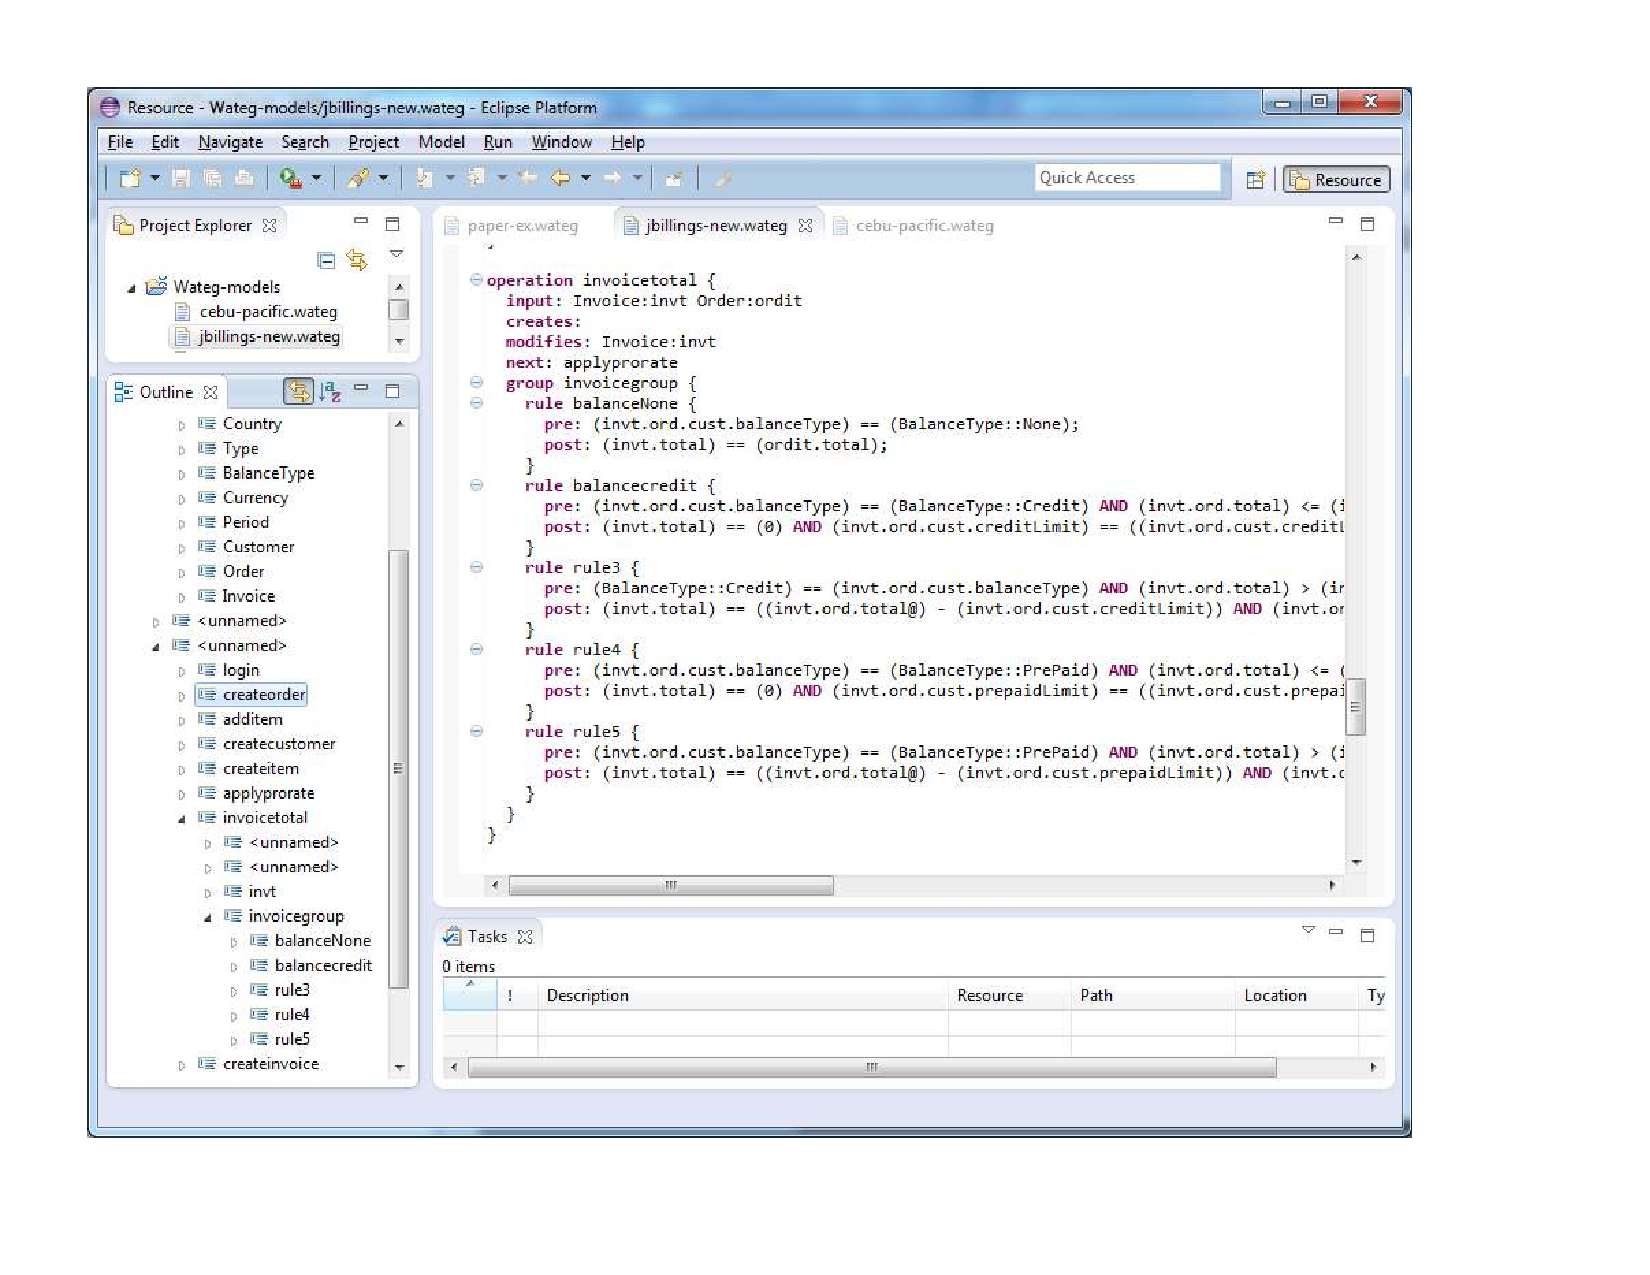
\includegraphics[trim=43 65 114 36,clip,width=\columnwidth]{figs/rule-editor.pdf}
\vspace*{-13pt}
\caption{Screenshot of the Eclipse-based rule editor.}
\vspace*{-0pt}
\label{fig:rule-editor}
\end{figure}

%% Our end goal of test generation requires accurate rule models. Moreover, we want
The modeling process must be realistic in that users should be able to create
and refine models in a tool-assisted manner, with immediate checking of, and
feedback on, errors in the models.  We have implemented such a rule editor as an
Eclipse plugin; Figure~\ref{fig:rule-editor} shows a screenshot of the
editor. The editor is built using Eclipse Xtext~\cite{xtext}, which is a general
framework for developing domain-specific and programming languages. Much like
any modern syntax-directed editor for a programming language, the rule editor
provides syntax highlighting, navigation features, auto completion, and
on-the-fly detection of syntax errors.  The user can also run a semantic checker
to detect violations of the well-formedness properties discussed
previously. Thus, the editor provides a convenient environment for writing
rules, in which the user is guided by automated checking and feedback.
